\documentclass{article}
\usepackage[utf8]{inputenc}
\usepackage{indentfirst}
\usepackage{amsmath}
\usepackage{amssymb}
\usepackage{pdfpages}
\usepackage [english]{babel}
\usepackage{minted} 
\usepackage [autostyle, english = american]{csquotes}
\MakeOuterQuote{"}
\allowdisplaybreaks 
\usepackage{atbegshi}% http://ctan.org/pkg/atbegshi
\AtBeginDocument{\AtBeginShipoutNext{\AtBeginShipoutDiscard}}




\begin{document}
\title{The Power Method, QR Method, and Deflation}
\author{Eli Slothower}
\date{December 9, 2022}
\maketitle
\setcounter{page}{1}

\section{Introduction}

It is well known that to find the eigenvalues, eigenvectors, singular values, and singular vectors of an $n \times n$ matrix $A$, one can start by calculating the roots of its characteristic polynomial, namely those of $A - \lambda I$, and assigning each root as an eigenvalue of $A$. From there, the eigenvectors, singular values, and singular vectors can be found through various other methods. However, finding the roots of the characteristic polynomial is far too slow of a process, even for computers, and, in fact, this method is impossible when $n > 4$.\textsuperscript{6} Iterative methods, such as the Power Method and the $QR$ Method, are much faster at calculating such things, and there aren't any restrictions how small or large $n$ must be. Even so, however, these methods can still be improved upon. The Power Method, for example, falls short in that it only computes the dominant eigenvalue, eigenvector, singular value, and singular vectors of a matrix, rather than \textit{all} eigenvalues, eigenvectors, et cetera. This paper and its accompanying software will explore these methods, as well as methods of improving the Power Method, and uncover how they work.

\section{The Power Method}
As stated above, the Power Method is an iterative method of calculating the dominate eigenvalue, eigenvector, singular value, and singular vectors of a matrix A. We will discuss later on how to find all values (rather than just the dominant values) of a matrix with the Power Method. Before looking at how the Power Method works, let us first define what it means to be an \textit{iterative} method. According to the Oxford Dictionary, iteration is defined as "the action of iterating or repeating, or process of being iterated."\textsuperscript{3} Thus we can conclude that an iterative method is one that repeats its process until it comes to its result.
\par The Power Method tells us that if $A$ is an $n \times n$ symmetric matrix with $n$ real, distinct eigenvalues, then the Power Method will return $\lambda_1$ where $|\lambda_1| > |\lambda_2| > ... > |\lambda_n|$.\textsuperscript{5, 6} There are still two main questions left to answer regarding this method though, namely (1) "How does this method work?", and (2) "Why does this method work?". Let us continue by answering the first question.
\par To begin, create a vector $\vec{x}^{\,}_0$ as an initial approximation of the dominant eigenvector of $A$.\textsuperscript{4} Next, find $\vec{x}^{\,}_1$ by computing $A\vec{x}^{\,}_0$. Next, find $\vec{x}^{\,}_2$ by computing $A\vec{x}^{\,}_1$. This is the point at which the \textit{iterative} process of the Power Method begins to show itself; continue this process to find $\vec{x}^{\,}_i$ for $0 \leq i \leq p$ where $p$ is an integer such that $A\vec{x}^{\,}_p$ converges to a point. Given a symmetric matrix $A$, as specified, the Power Method will always converge to a point. Once $\vec{x}^{\,}_p$ has been calculated, the dominant eigenvalue, $\lambda_1$, can be found by calculating $\frac{\vec{x}^{\,T}_p\vec{x}^{\,}_{p+1}}{\vec{x}^{\,T}_p\vec{x}^{\,}_{p}}$.\textsuperscript{5} The dominant eigenvalue has now been found, and the eigenvectors, singular values, and singular vectors can now be found from here, which we will discuss how to do later.
\par Why does this method work? When we look at the proof, it becomes clear. \\\\

\noindent \textbf{Lemma 1:} $\lim_{p\to\infty} \sum_{i=2}^{n} c_i(\frac{\lambda_i}{\lambda_1})^pe_i = 0$ because as $p$ increases, $|\lambda_1|^p > |\lambda_i|^p$ since $\lambda_1$ is the leading eigenvalue of $A$, so $\lim_{p\to\infty} (\frac{\lambda_i}{\lambda_1})^p = 0$.
\\\\

\noindent \textbf{Theorem 1:}\textsuperscript{5, 6} If $A$ is an $n \times n$ symmetric matrix with $n$ real, distinct eigenvalues, then the Power Method will return the dominant eigenvalue of $A$, denoted as $\lambda_1$. \\\\

\noindent Let $\vec{x}^{\,}_0 \in R^n$ as an initial approximation of the dominant eigenvector. Because $A$ has $n$ distinct eigenvalues, we know that $A$ has $n$ linearly independent eigenvectors. Thus, let us represent $\vec{x}^{\,}_0$ as a linear combination of the eigenvectors, $e_i$, with constants $c_i$.

\begin{align*}
    \text{Let } \vec{x}^{\,}_0 &= c_1e_1 + c_2e_2 + ... + c_ne_n \tag{i.e. an approximation of one of the dominant eigenvectors of $A$}\\
    &=\sum_{i=1}^{n} c_ie_i \tag{by summation form}\\\\
    \text{Let }\vec{x}^{\,}_1 &= A\vec{x}^{\,}_0\\
    &=A\sum_{i=1}^{n} c_ie_i \tag{by summation form}\\
    &=\sum_{i=1}^{n} c_iAe_i \tag{by linearity}\\
    &=\sum_{i=1}^{n} c_i\lambda_i e_i \tag{by $Ae_i = \lambda_i e_i$}\\\\
    \text{Let }\vec{x}^{\,}_p &= A^p\vec{x}^{\,}_0\\
    &= \sum_{i=1}^{n} c_i\lambda^p_i e_i \tag{by powers of a diagonalizable matrix}\\
    &=c_1\lambda^p_1e_1 + \sum_{i=2}^{n} c_i\lambda^p_i e_i \tag{by factorization}\\  
    &=\lambda^p_1(c_1e_1 + \sum_{i=2}^{n} c_i(\frac{\lambda_i}{\lambda_1})^pe_i) \tag{by factorization}\\ 
    \implies \vec{x}^{\,}_p = \lambda^p_1(c_1e_1 + \sum_{i=2}^{n} c_i(\frac{\lambda_i}{\lambda_1})^pe_i) &\approx \lambda^p_1c_1e_1\tag{by Lemma 1}\\
    \implies x_{p+1} &\approx\lambda^{p+1}_1c_1e_1\\\\
    \text{Then, }\frac{\vec{x}^{\,T}_p\vec{x}^{\,}_{p+1}}{\vec{x}^{\,T}_p\vec{x}^{\,}_{p}} &= \frac{(c_1\lambda^p_1e^T_1)(c_1\lambda^{p+1}_1e_1)}{(c_1\lambda^p_1e^T_1)(c_1\lambda^p_1e_1)}\tag{by substitution}\\
    &=\frac{e^T_1\lambda_1e_1}{e^T_1e_1}\tag{by division of constants}\\
    &=\frac{\lambda_1e^T_1e_1}{e^T_1e_1}\tag{by linearity}\\
    &=\lambda_1 \tag{by division of constants (dot product of $e^T_1e_1$ results in a constant)}\\\\
    \therefore \text{By the Power Method, }\lambda_1 = \frac{\vec{x}^{\,T}_p\vec{x}^{\,}_{p+1}}{\vec{x}^{\,T}_p\vec{x}^{\,}_{p}}
\end{align*}
\begin{flushright}
    $\square$
\end{flushright}

\noindent Now let us discuss how to find the dominant eigenvector, dominant singular value, and dominant singular vectors from the Power Method. \\\\

\noindent\textbf{1). }Let $s$ be the maximum component in $\vec{x}^{\,}_{p}$. Then, from the Power Method, the dominant eigenvector of $A$ is $\vec{x}^{\,}_{p}$ by definition of $\vec{x}^{\,}_{p}$.\\

\noindent\textbf{2). } Let $\lambda_1$ be the dominant eigenvalue of $A$ returned from the Power Method. Then the dominant singular value of $A$ is $\sqrt{\lambda_1}$, by definition of singular value. \\

\noindent\textbf{3). } Let $\vec{x}_{p, A^TA}$ be the dominant eigenvector of $A^TA$ returned from the Power Method. Then the dominant right singular vector of $A$ is $\lambda_{1, A^TA}$, by definition of right singular vector. \\

\noindent\textbf{4). } Let $\vec{x}_{p, AA^T}$ be the dominant eigenvector of $AA^T$ returned from the Power Method. Then the dominant left singular vector of $A$ is $\lambda_{1, AA^T}$, by definition of left singular vector. \\

\noindent Now that we know both how the Power Method works and why the Power Method works, let us take a look at the accompanied software to gain some more intuition about the code, as well as the provided examples. \\

\noindent \textit{Note: Before continuing, please refer to the appendix and review all necessary functions and examples. Note that all of our Power Method functions take in a matrix $A$ that abides by the preconditions, as well as an $n \times 1$ initial approximation x.}\\

\noindent \textbf{Example PM.1: }This is a trivial case. The purpose of this example is to show that our function works on trivial cases. We know that the dominant eigenvalue is 2 since $A$ is a diagonal matrix. This is what our getEvaluePM(A,x) returns. We know that the corresponding eigenvector is [1, 0], which is what our getEvectorPM(A, x) returns. Next, we know the corresponding singular value should be $\sqrt2$, which is what our getSingularValuePM(A,x) returns. Lastly, our getSingularVectorAtAPM(A,x) and getSingularVectorAAtPM(A,x) correctly return the left
and right singular vectors, which we can verify with a singular vector calculator.\\

\noindent \textbf{Example PM.2: }This is a non-trivial case, although it is not an extremely difficult one. The purpose of this example is to show that our function works on normal-difficulty cases. Using an eigenvalue calculator, we can see that the dominant eigenvalue of $A$ is 17.034, which our getEvaluePM(A,x) returns. Similarly, we know that the dominant eigenvector of $A$ is [0.577; 0.547; 0.606], which our getEvectorPM(A,x) returns. Our getSingularValuePM(A,x) properly returns $\sqrt{17.034}$, which we would expect. Lastly, our  getSingularVectorAtAPM(A,x) and getSingularVectorAAtPM(A,x) properly returns the dominant singular vector that a singular vector calculator returns.\\

\noindent \textbf{Example PM.2.1: }This is an extension of Example PM.2. The purpose of this example is to show that our intitial approximation $\vec{x}$ can truly be arbitrary (with the appropriate dimensions of course), and we still get the expected results with all of our functions. As we can see, all results in this example are the same as the results in that of Example PM.2, which we would expect.\\

\noindent \textbf{Example PM.3: }This is a non-trivial, difficult case. The purpose of this example is to show that our functions work on large matrices. To be said succinctly, all five of our Power Method functions properly return the expected answers for this large matrix, which we can verify with various calculators.\\

\noindent We have now shown that our Power Method functions work on trivial and non-trivial cases.

\section{The $QR$ Method}
In its current form, we can see that the Power Method isn't as useful as we want it to be; we would like to be able to find \textit{all} eigenvalues, eigenvectors, singular values, and singular vectors of a matrix. It is here at which the $QR$ Method becomes useful. The $QR$ Method tells us that if we have an $n \times n$ real matrix $A$, then we will come to a (nearly) upper-triangular matrix $A_k$ that contains approximations to the eigenvalues of $A$ on the diagonal.\textsuperscript{2} We say that it is "nearly" upper-triangular because the components below the diagonal will either converge to 0, or become negligible ($\sim$  $>$0.1) Again, we are left with two main questions to answer regarding this method, namely (1) "How does this method work?", and (2) "Why does this method work?". Let us continue by answering the first question.
\par To start, use $QR$ decomposition to factor $A$ into $Q_1R_1$. Then let $A_1 = R_1Q_1$. Next, use $QR$ decomposition to factor $A_1$ into $Q_2R_2$. Then let $A_2 = R_2Q_2$. It is at this point that the iterative process becomes clear; continue this process until $A_k$ seems to converge, as described above. Once it does, the elements on the diagonal of $A_k$ will be the eigenvalues of $A$.\textsuperscript{2, 6}
\par Why does this method work? Let us take a look at the proof.\\

\noindent \textbf{Theorem 2:}\textsuperscript{6} If $A$ is an $n \times n$ nonsingular matrix, then the QR Method will return a matrix with its eigevalues equal to those of the eigenvalues of $A$. \\

\noindent Note: We will assume that the matrix the $QR$ Method returns is an upper-triangular matrix, meaning that its eigenvalues are the components on its diagonal. We will not be proving in this paper why the $QR$ Method returns a matrix that converges into such a matrix; we are instead simply proving that its eigenvalues are equal to those of $A$. \\

\noindent Let $A$ be an $n \times x$ nonsingular matrix.



\begin{align*}
    A &= Q_1R_1\tag{by QR decomposition}\\\\
    \text{Let } A_1 &= R_1Q_1\\
    \intertext{Note: $A_1$ has the same eigenvalues as $A$ because $A = Q_1R_1$ is similar to $A_1$ = $Q^{-1}AQ$. We know $Q^{-1}$ exists because, by Gram-Schmidt, $Q$ is an orthogonal matrix.}
    A_1 &= Q_2R_2 \tag{by QR decomposition}\\
    \text{Let } A_2 &= R_2Q_2\\
    \intertext{Note: $A_2$ has the same eigenvalues as $A_1$ due to the same logic as explained above.}\\
    \text{Let } A_p &= R_pQ_p \: \: \: \forall \: p \in \mathbb{N}
    \intertext{Note: $A_p$ has the same eigenvalues as $A$ due to the same logic as explained above.}
    \intertext{Recall that $A_p$ is assumed to be an upper-triangular matrix.}
\end{align*}

\noindent$\therefore$ \text{By the QR Method, the eigenvalues of $A_p$ are equal to those of the}\\\text{\:\:\:\:\:eigenvalues of $A$.}

\begin{flushright}
    $\square$
\end{flushright}

\noindent Now that we know both how the $QR$ Method works and why the $QR$ Method works, let us take a look at the accompanied software to gain some more intuition about the code, as well as the provided examples. \\

\noindent \textit{Note: Before continuing, please refer to the appendix and review all necessary functions and examples. Note that all of our $QR$ Method functions take in a matrix $A$ that abides by the preconditions.}\\

\noindent \textbf{Example QR.1: }This is the trivial case. The purpose of this example is to show that our function works on trivial cases. We know that since $A$ is a diagonal matrix, its eigenvalues are on the diagonal. Luckily, our getEvaluesQR(A) correctly returns 2 and 1 as our eigenvalues. We also know that the eigenvectors of $A$ are [1,0] and [0,1], which our getEvectorsQR(A) correctly returns. Furthermore, our getSingularValuesQR(A) correctly returns $\sqrt2$ and $\sqrt1$, which makes sense since 2 and 1 are the eigenvalues of $A$. Lastly, our getLeftSingularVectorsQR(A) and getRightSingularVectorsQR(A) correctly return the left and right singular vectors, which we can verify with a singular vector calculator.\\

\noindent \textbf{Example QR.2: }This is a non-trivial case, although it is not an extremely difficult one. The purpose of this example is to show that our function works on normal-difficulty cases. Using an eigenvalue calculator, we can see that the eigenvalues of $A$ are 17.034, -2.561, and 0.527. Our getEvaluesQR(A) returns these same results. Similarly, our getEvectorsQR(A) returns the same results as an eigenvector calculator. Next, our getSingularValuesQR(A) correctly returns the square roots of each of the eigenvalues we calculated. Our getLeftSingularVectorsQR(A) and getRightSingularVectorsQR(A) both return correct values as well, according to singular vector calculators. \\

\noindent \textbf{Example QR.3: }This is a non-trivial, difficult case. The purpose of this example is to show that our functions work on large matrices. To be said succinctly, all five of our $QR$ functions properly return the expected answers for this large matrix, which we can verify with various calculators.. \\

\noindent We have now shown that our $QR$ functions work on trivial and non-trivial cases.

\section{Deflation}
Recall that the Power Method only helps us find the dominant eigenvalue, dominant eigenvector, dominant singular value, and dominant left/right singular vectors of an $n \times n$ symmetric matrix A. Usually though, we want to find \textit{all} of these values, not just the dominant ones. Luckily, this is possible by improving upon the Power Method with a process known as "deflation."  
\par The purpose of deflation is to "modify a matrix to eliminate the influence of a given eigenvector, typically by setting the associated eigenvalue to zero."\textsuperscript{1} Applying this method to the Power Method, we can easily find all eigenvalues of a matrix A that satisfies the preconditions of the Power Method (and the following eigenvectors, singular values, and singular vectors).
\par How does this method work? Begin with an $n \times x$ matrix $A$ that satisfies the preconditions of the Power Method. Use the Power Method to calculate the dominant eigenvalue (denoted as $\lambda_1$), dominant eigenvector (denoted as $v_1$), dominant singular value, and dominant singular vectors. Next, let $A_1 = A - \frac{\lambda_1}{(\vec{v}^{T}\vec{v})^2} \vec{v}\vec{v}^{T}$. This eliminates the influence of the dominant eigenvector, $\vec{v}_1$, and zeros out its associated eigenvalue from the matrix. Now, call the Power Method on $A_1$, which will return its dominant eigenvalue (denoted as $\lambda_2$), dominant eigenvector (denoted as $v_2$), dominant singular value, and dominant singular vectors. Create $A_2$ using the same formula, but with $A_1$, $\lambda_2$, and $\vec{v}_2$. It is at this point that the iterative process becomes clear; continue this process up to and including $A_{n-1}$, for which at this point all desired values will have been computed.\textsuperscript{7} \\

\noindent Now that we know how deflation with the Power Method works, let us take a look at the accompanied software to gain some more intuition about the code, as well as the provided examples. Note that all of our Power Method and Power Method Deflation functions take in a matrix $A$ that abides by the preconditions, as well as an $n \times 1$ initial approximation x.\\

\noindent \textit{Note: Before continuing, please refer to the appendix and review all necessary functions and examples.}\\

\noindent \textbf{Example PMD.1: }This is the trivial case. The purpose of this example is to show that our function works on trivial cases. We expect that our Power Method Deflation functions would return the same results as our $QR$ Method functions would (even though both methods use completely different algorithms) since the $QR$ Method and the Power Method with deflation return the same things (i.e. all eigenvalues, eigenvectors, singular values, and singular vectors). Luckily, all five of our Power Method Deflation functions return the same thing as our $QR$ Method functions in Example QR.1.\\

\noindent \textbf{Example PMD.2: }This is a non-trivial case, although it is not an extremely difficult one. The purpose of this example is to show that our function works on normal-difficulty cases. Knowing that our five Power Method Deflation functions return the same results as our $QR$ Method functions in Example QR.2, and using the reasoning we explained above in Example PMD.1, we know our Power Method Deflation functions work properly for this example.\\

\noindent \textbf{Example PMD.3: }This is a non-trivial, difficult case. The purpose of this example is to show that our functions work on large matrices. Knowing that our five Power Method Deflation functions return the same results as our $QR$ Method functions in Example QR.3, and using the reasoning we explained above in Example PMD.1, we know our Power Method Deflation functions work properly for this example. \\

\noindent We have now shown that our Power Method Deflation functions work on trivial and non-trivial cases.



\begin{thebibliography}{5}
%
\bibitem {def}
{\it Deflation methods for sparse PCA}. deflation Methods for Sparse PCA - statwiki. (n.d.). Retrieved December 9, 2022, from https://wiki.math.uwaterloo.ca/statwiki/index.php?title=deflation\_\\Methods\_for\_Sparse\_PCA 

\bibitem {gil}
Gilbert Strang - MIT. (2019). {\it Computing Eigenvalues and Singular Values. YouTube}. Retrieved December 6, 2022, from https://youtu.be/d32WV1rKoVk.

\bibitem {ite}
{\it Iteration}. Home : Oxford English Dictionary. (n.d.). Retrieved December 6, 2022, from https://www.oed.com/view/Entry/100312?redirectedFrom=iteration

\bibitem {jef}
Jeffrey Chasnov. (2021). {\it Eigenvalue Power Method (Example) | Lecture 31 | Numerical Methods for Engineers. YouTube}. Retrieved December 6, 2022, from https://youtu.be/nKd0lu3yThg. 

\bibitem {jef}
Jeffrey Chasnov. (2021). {\it Eigenvalue Power Method | Lecture 30 | Numerical Methods for Engineers. YouTube}. Retrieved December 6, 2022, from bit.ly/3Y2SfvC. 

\bibitem {str}
Strang, G. (2021). {\it Introduction to linear algebra}. Wellesley-Cambridge Press.

\bibitem {you}
{\it YouTube. Lecture 47 Matrix Eigenvalue Problems - 2 Power Method - 2}. Retrieved December 9, 2022, from https://youtu.be/WVA6pVtMFgs. 

\end{thebibliography}

\section{Appendix}

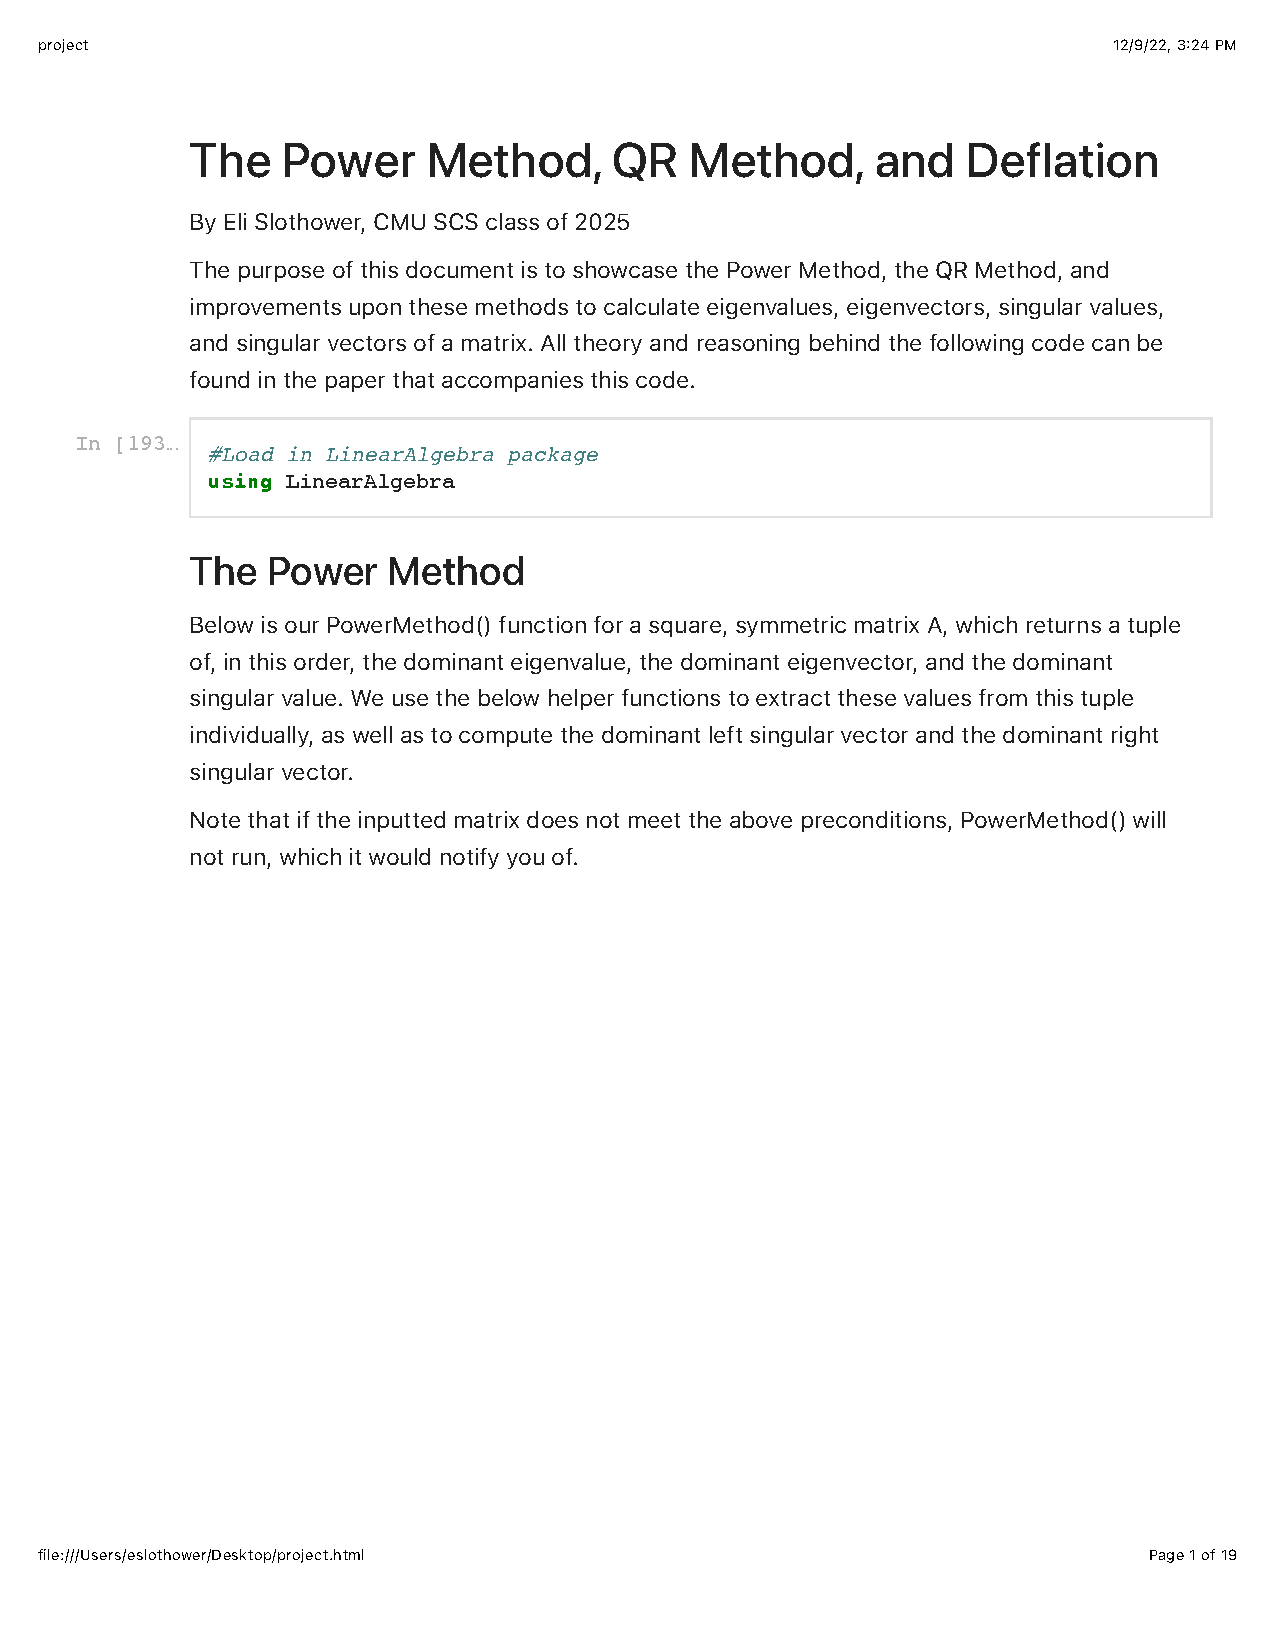
\includepdf[pages=-]{project.pdf}

\end{document}
